% LPPLS-kuplaskanneri: teoria ja havaitsemisen ehdot
% Käännös:  (kuvat valmiina kansiossa fig/)
%           cd docs && latexmk -pdf LPPLS_kuplaskanneri_teoria.tex
\documentclass[10pt,a4paper]{article}

\usepackage[T1]{fontenc}
\usepackage[utf8]{inputenc}
\usepackage[finnish]{babel}
\usepackage{lmodern}
\usepackage{microtype}
\usepackage[a4paper,left=2.3cm,right=2.3cm,top=2.0cm,bottom=2.0cm]{geometry}
\usepackage{amsmath,amssymb,bm}
\usepackage{graphicx}
\usepackage{booktabs,tabularx,array}
\usepackage[font=small,labelfont=bf,labelsep=period]{caption}
\usepackage{fancyhdr}
\usepackage{xcolor}
\usepackage[authoryear,round]{natbib}
\usepackage[hidelinks,pdfusetitle]{hyperref}
\usepackage{url}
\usepackage[autostyle]{csquotes}

\setcitestyle{aysep={},yysep={,}}
\graphicspath{{fig/}}
\addto\captionsfinnish{\renewcommand{\refname}{Lähteet}}
\definecolor{navy}{HTML}{1F2A44}
\captionsetup[table]{position=below}
\renewcommand{\arraystretch}{1.15}

\pagestyle{fancy}
\fancyhf{}
\fancyhead[L]{\small\color{gray}LPPLS-kuplaskanneri -- teoria ja havaitsemisen ehdot}
\fancyfoot[C]{\small\color{gray}\thepage}
\renewcommand{\headrulewidth}{0pt}
\fancypagestyle{plain}{\fancyhf{}\fancyfoot[C]{\small\color{gray}\thepage}}

\newcommand{\tc}{t_c}
\newcommand{\pv}{\,\mathrm{pv}}

\title{\color{navy}\textbf{LPPLS-kuplaskanneri}\\[4pt]
  \large\mdseries Teoria, hintadatan käyttö ja kuplien havaitsemisen ehdot}
\author{}
\date{}

\hypersetup{pdftitle={LPPLS-kuplaskanneri: teoria ja havaitsemisen ehdot},
  pdfauthor={LPPLS-kuplaskanneri},
  pdfsubject={LPPLS-malli ja kuplien havaitseminen}}

\begin{document}
\maketitle
\vspace{-3.5em}
\thispagestyle{plain}

\begin{abstract}
\noindent
Tässä dokumentissa kuvataan LPPLS-kuplaskanneri, Pythonilla toteutettu työpöytäsovellus, joka
etsii osake-, raaka-aine- ja kryptomarkkinoilta kuplia ennen kuin ne puhkeavat. Tavoitteena on
korvata jälkikäteen tehtävä arvio ennakoivalla, toistettavalla ja läpinäkyvällä menetelmällä,
jonka jokainen raja-arvo on perusteltu kirjallisuudella. Sovelluksen perustana on Didier
Sornetten ja kollegoiden kehittämä LPPLS-malli (\emph{log-periodic power law singularity}).
Mallin mukaan sijoittajien laumakäyttäytyminen saa kuplan aikana hinnan kasvamaan nopeammin kuin
eksponentiaalisesti. Kasvu kiihtyy kohti kriittistä hetkeä~$\tc$, jolloin romahduksen
todennäköisyys on suurimmillaan, ja kiihtyvään trendiin liittyy log-periodisia värähtelyjä,
jotka tihenevät $\tc$:tä lähestyttäessä. Sovellus hakee jokaiselle seurattavalle tunnukselle
noin neljän vuoden päivittäiset päätöskurssit Yahoo Financesta ja sovittaa mallin hintojen
logaritmeihin 24 eri pituisessa aikaikkunassa (puolesta vuodesta neljään vuoteen), jotka kaikki
päättyvät tarkastelupäivään. Sovitus tehdään Filimonovin ja Sornetten menetelmällä: neljä
lineaarista parametria ratkaistaan suoraan pienimmän neliösumman menetelmällä, ja vain kolme
epälineaarista parametria haetaan numeerisesti. Jokainen sovitus tarkistetaan kirjallisuudesta
poimituilla ehdoilla. Niiden ikkunoiden osuus, jotka läpäisevät ehdot ja ennustavat $\tc$:n
puolen vuoden sisään, muodostaa luottamusindikaattorin. Tilanne luokitellaan kuplaksi, kun
luottamusindikaattori on vähintään 10\,\% ja hinta on lisäksi vähintään kaksinkertaistunut
kahdessa vuodessa. Jälkimmäinen ehto perustuu Greenwoodin, Shleiferin ja Youn havaintoon, että
näin suuri nousu nostaa romahduksen todennäköisyyden yli puoleen. Havaitut kuplat tallennetaan
tietokantaan, ja sovellus seuraa, toteutuiko ennustettu käänne: kupla katsotaan toteutuneeksi,
jos ennustetun hetken lähellä tulee huippu ja sitä seuraa vähintään 15\,\%:n pudotus. Ehtoja
testattiin historiallisilla kuplilla, kuten Bitcoinin vuoden 2017, Shanghain pörssin vuosien
2007 ja 2015 sekä Nasdaqin vuoden 2000 kuplilla, ja ne tunnistivat kuusi kahdeksasta.
Kriittisen hetken arvio osui 0--4 viikon päähän todellisesta huipusta. Menetelmä on tutkimuksen
ja opiskelun väline, ei sijoitussuositus.
\end{abstract}

% ---------------------------------------------------------------------------
\section{Johdanto}

Rahoitusmarkkinoiden kupla on tilanne, jossa hinta irtoaa perustekijöistään ja nousee
itseään ruokkivasti: nousu houkuttelee uusia ostajia, jotka nostavat hintaa edelleen. Kuplat
tunnistetaan yleensä vasta jälkikäteen, kun romahdus on jo tapahtunut. Sornette esittää, että
kuplilla on mitattava \enquote{sormenjälki}: hinta kasvaa nopeammin kuin eksponentiaalisesti, ja
kasvuun liittyy tiheneviä värähtelyjä \citep{sornette2003,johansen2010}. Jos sormenjälki löytyy
hintasarjasta ajoissa, kuplan loppumisajankohtaa voidaan arvioida etukäteen.

LPPLS-kuplaskanneri soveltaa tätä ajatusta järjestelmällisesti. Sovellus käy läpi
seurantalistan (oletuksena 75 osakeindeksiä, 39 raaka-ainefutuuria, 40 suurinta kryptovaluuttaa
sekä 41 teemarahastoa, osaketta ja sektoria), sovittaa mallin jokaiseen sarjaan, luokittelee
tuloksen ja tallentaa havaitut kuplat. Myöhemmin se hakee uutta dataa ja tarkistaa, toteutuiko
ennuste. Luvussa~\ref{sec:teoria} esitellään mallin teoria, luvussa~\ref{sec:data} kuvataan,
miten hintadataa käytetään parametrien estimointiin, luvussa~\ref{sec:ehdot} käydään läpi
kuplan ehdot, ja luvussa~\ref{sec:kalibrointi} arvioidaan menetelmän osuvuutta ja rajoituksia.

% ---------------------------------------------------------------------------
\section{Mallin teoria}\label{sec:teoria}

\subsection{Rationaalinen kupla ja romahdusriski}

LPPLS-malli pohjautuu Johansenin, Ledoit'n ja Sornetten JLS-malliin \citep{johansen2000}.
Siinä hinta $p$ noudattaa prosessia
\begin{equation}\label{eq:jls}
  \frac{dp}{p} = \mu(t)\,dt + \sigma(t)\,dW - \kappa\,dj,
\end{equation}
missä $\mu$ on hinnan odotettu kasvuvauhti, $\sigma\,dW$ satunnaista vaihtelua ja $j$
hyppyprosessi, joka saa arvon 1 romahduksen sattuessa. Romahdus pudottaa hintaa osuuden
$\kappa$. Romahduksen todennäköisyyttä aikayksikköä kohden kuvaa riskifunktio $h(t)$. Mallissa
sijoittajat ovat rationaalisia: niin kauan kuin romahdusta ei ole tapahtunut, hinnan odotettu
muutos on nolla (arbitraasittomuus). Tästä seuraa
\begin{equation}\label{eq:arb}
  \mathrm{E}[dp] = 0 \quad\Longrightarrow\quad \mu(t) = \kappa\, h(t).
\end{equation}
Hinnan on siis noustava sitä nopeammin, mitä suurempi romahdusriski on, jotta sijoittajat
saavat korvauksen riskin kantamisesta. Kuplan aikana riski kasvaa, koska sijoittajat matkivat
toisiaan: laumakäyttäytyminen voimistuu, kunnes yhä suurempi osa markkinasta toimii samaan
suuntaan. Ilmiö muistuttaa fysiikan faasimuutosta, jossa järjestelmä lähestyy kriittistä
pistettä. Kun sijoittajien vuorovaikutusverkostolla on hierarkkinen rakenne, riskifunktio saa
muodon
\begin{equation}\label{eq:hazard}
  h(t) \approx B'\,(\tc-t)^{m-1} + C'\,(\tc-t)^{m-1}\cos\!\bigl(\omega \ln(\tc-t) - \phi'\bigr).
\end{equation}
Integroimalla yhtälön~\eqref{eq:arb} kasvuvauhti ajan yli saadaan odotetulle log-hinnalle
LPPLS-yhtälö
\begin{equation}\label{eq:lppls}
  \ln \mathrm{E}[p(t)] = A + B\,(\tc-t)^m + C\,(\tc-t)^m \cos\!\bigl(\omega\ln(\tc-t)-\phi\bigr),
  \qquad t<\tc .
\end{equation}

\subsection{Parametrien tulkinta}

$\bm{\tc}$ on kriittinen hetki eli kuplan todennäköisin loppumisajankohta. Se ei ole varma
romahduspäivä: \citet{johansen2010} arvioivat, että noin kolmasosa kuplista päättyy pehmeään
laskuun ilman romahdusta. $\bm{m}\in(0,1)$ kuvaa kiihtyvyyttä. Log-hinnan kasvuvauhti on
$-mB(\tc-t)^{m-1}$, ja se kasvaa rajatta, kun $t\to\tc$. Itse hinta pysyy silti äärellisenä, ja
tätä kutsutaan äärellisen ajan singulariteetiksi. $\bm{B}<0$ tarkoittaa kiihtyvää nousua eli
positiivista kuplaa, ja $B>0$ kiihtyvää laskua eli antikuplaa. $\bm{\omega}$ on värähtelyjen
log-taajuus: peräkkäisten värähtelyjen etäisyydet $\tc$:stä pienenevät suhteessa
$\lambda = e^{2\pi/\omega}$, joten esimerkiksi arvolla $\omega = 9$ jokainen jakso on noin
puolet edellisestä. $\bm{C}$ ja $\bm{\phi}$ ovat värähtelyn amplitudi ja vaihe, ja $\bm{A}$ on
log-hinta hetkellä~$\tc$. Kuva~\ref{fig:malli} havainnollistaa mallin osia.

\begin{figure}[htbp]
  \centering
  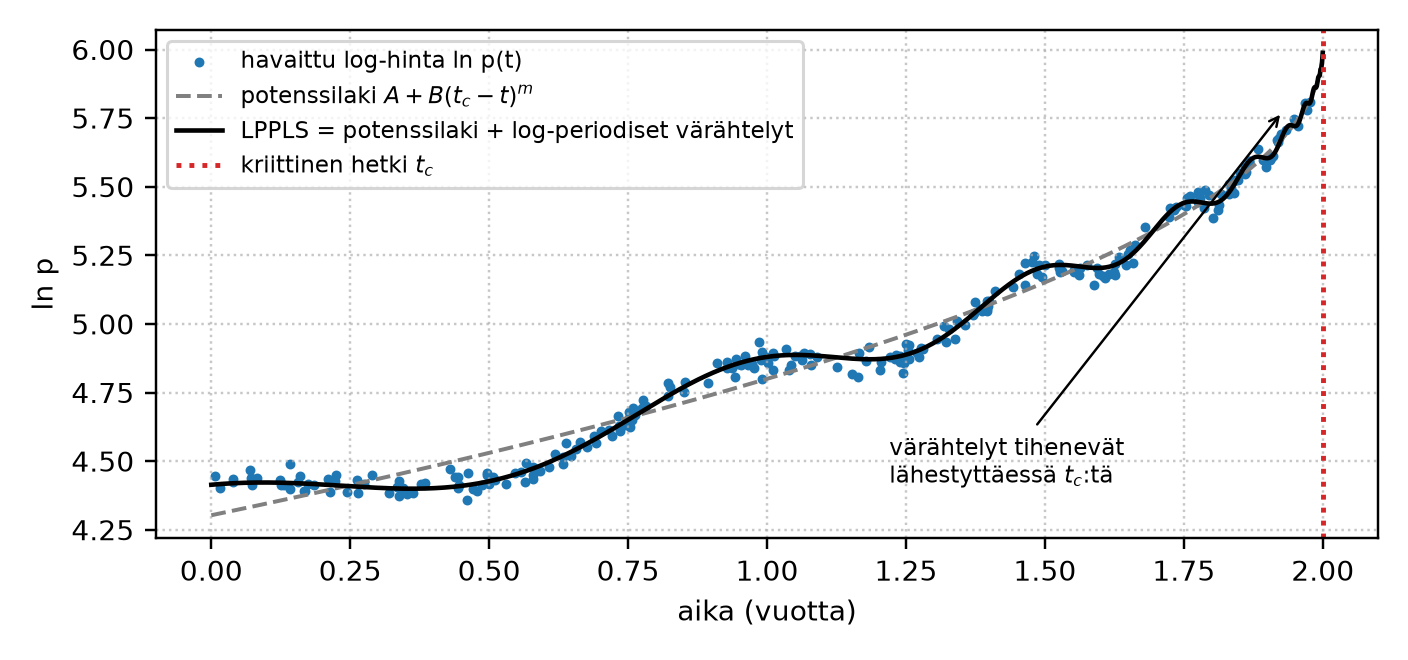
\includegraphics[width=0.72\textwidth]{kuva1_malli.png}
  \caption{Synteettinen LPPLS-kupla. Katkoviiva on pelkkä potenssilakitrendi, ja musta käyrä
    lisää siihen log-periodiset värähtelyt. Siniset pisteet ovat kohinaisia
    \enquote{havaintoja}. Kasvu kiihtyy ja värähtelyt tihenevät kohti kriittistä
    hetkeä~$\tc$.}
  \label{fig:malli}
\end{figure}

% ---------------------------------------------------------------------------
\section{Miten hintadataa käytetään estimointiin}\label{sec:data}

\subsection{Aineisto}

Sovellus hakee Yahoo Financesta päivittäiset päätöskurssit, jotka on korjattu osingoilla ja
osakesplittauksilla. Data haetaan noin neljän vuoden ajalta tarkastelupäivään $t_2$ asti.
Malliin syötetään hintojen logaritmit $y_i = \ln p_i$ hetkillä $t_i$, jotka on ilmaistu
desimaalivuosina. Logaritmin ansiosta suhteelliset muutokset ovat samassa mittakaavassa
riippumatta hintatasosta. Malli näkee vain hetkeä $t_2$ edeltävän datan, joten arvio on aidosti
ennakoiva. Testitilassa $t_2$ voidaan asettaa menneisyyteen, jolloin historiallisia kuplia voi
tutkia ilman, että malli \enquote{näkee} tulevaisuutta. Haettu data tallennetaan
SQLite-välimuistiin.

\subsection{Sovitus linearisoimalla}

Yhtälössä~\eqref{eq:lppls} on seitsemän parametria, ja niiden suora optimointi on epävakaata,
koska virhefunktiolla on paljon paikallisia minimejä. \citet{filimonov2013} kirjoittavat
kosinitermin uudelleen muotoon
\begin{equation}\label{eq:linear}
  \begin{gathered}
  y(t) = A + B f(t) + C_1 g(t) + C_2 k(t),\\
  f=(\tc-t)^m,\qquad g=f\cos\bigl(\omega\ln(\tc-t)\bigr),\qquad k=f\sin\bigl(\omega\ln(\tc-t)\bigr),
  \end{gathered}
\end{equation}
missä $C_1 = C\cos\phi$ ja $C_2 = C\sin\phi$. Kun epälineaariset parametrit $(\tc, m, \omega)$
on kiinnitetty, malli on lineaarinen parametrien $\bm{\beta} = (A, B, C_1, C_2)$ suhteen, ja
ne saadaan suoraan pienimmän neliösumman ratkaisuna:
\begin{equation}\label{eq:ols}
  \mathbf{y} = X\bm{\beta} + \bm{\varepsilon},\qquad
  X_i = \bigl[1,\ f_i,\ g_i,\ k_i\bigr],\qquad
  \hat{\bm{\beta}} = (X^{\top}X)^{-1}X^{\top}\mathbf{y}.
\end{equation}
Numeerisesti on siis haettava vain kolme parametria minimoimalla jäännösneliösumma:
\begin{equation}\label{eq:argmin}
  (\hat t_c,\hat m,\hat\omega) = \arg\min\, F(\tc,m,\omega),\qquad
  F = \sum_{i=1}^{N}\bigl(y_i - X_i\hat{\bm{\beta}}\bigr)^2 .
\end{equation}
Sovellus käyttää Nelder--Mead-simpleksimenetelmää \citep{nelder1965} kymmenestä satunnaisesta
alkupisteestä ja valitsee niistä pienimmän $F$:n. Hakualue on $m\in[0.01, 0.99]$,
$\omega\in[2, 25]$ ja $t_2 < \tc \le t_2 + 0.2\,\Delta t$, missä $\Delta t = t_2 - t_1$ on
ikkunan pituus \citep{zhang2016}. Hakualue on tarkoituksella väljempi kuin
luvun~\ref{sec:ehdot} hyväksymisehdot, jotta optimi ei jää keinotekoisesti rajalle. Koska $\tc$
rajataan tulevaisuuteen, malli etsii vain kuplia, jotka eivät ole vielä päättyneet.

\subsection{Monta ikkunaa ja luottamusindikaattori}

Yksittäinen sovitus on herkkä sille, mistä päivästä aikaikkuna alkaa, koska kuplan alkuhetkeä ei
tunneta. Siksi sovitus tehdään 24 ikkunaan, joiden pituudet ovat tasavälein 125, 163, 202,
\ldots, 1008 kauppapäivää (noin puolesta vuodesta neljään vuoteen; lyhin ikkuna kuten
\citealp{zhang2016}) ja jotka kaikki päättyvät hetkeen $t_2$. Jokainen ikkuna antaa oman arvionsa
parametreista. Luottamusindikaattori (\emph{LPPLS confidence}) on niiden ikkunoiden osuus, joiden
sovitus läpäisee luvun~\ref{sec:suodatin} suodattimen ja joiden $\tc$ osuu horisontin
$H = 6$~kk sisään:
\begin{equation}\label{eq:ci}
  \mathrm{CI}(t_2) = \frac{1}{K}\sum_{k=1}^{K}
  \mathbf{1}\!\left[\,\text{sovitus } k \text{ hyväksytty} \ \wedge\ t_2 < \tc^{(k)} \le t_2 + H\,\right].
\end{equation}
Hyväksyttyjen ikkunoiden $\tc$-arvioista lasketaan mediaani sekä 10\,\%:n ja 90\,\%:n
prosenttipisteet, jotka muodostavat ennustevälin. Kuvaan piirretään sovitus, jonka $\tc$ on
lähimpänä mediaania. Kuvissa~\ref{fig:shanghai} ja~\ref{fig:ikkunat} menetelmää on sovellettu
Shanghain pörssin vuoden 2015 kuplaan tilanteessa 1.6.2015.

\begin{figure}[htbp]
  \centering
  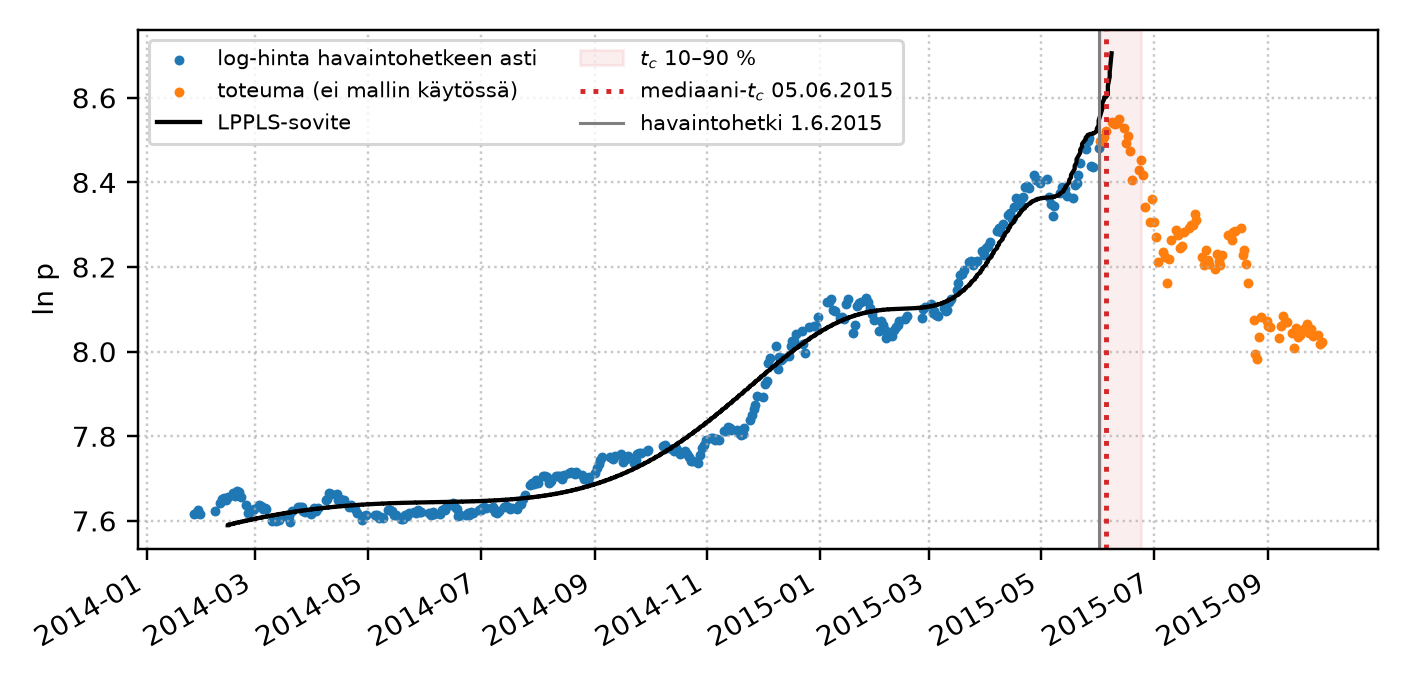
\includegraphics[width=0.72\textwidth]{kuva2_shanghai.png}
  \caption{Shanghai Composite, tarkastelupäivä 1.6.2015. Malli käytti vain sinisiä pisteitä.
    Mediaani-$\tc$ oli 5.6.2015, ja todellinen huippu tuli 12.6.2015, minkä jälkeen indeksi laski
    yli 40\,\% (oranssit pisteet).}
  \label{fig:shanghai}
\end{figure}

\begin{figure}[htbp]
  \centering
  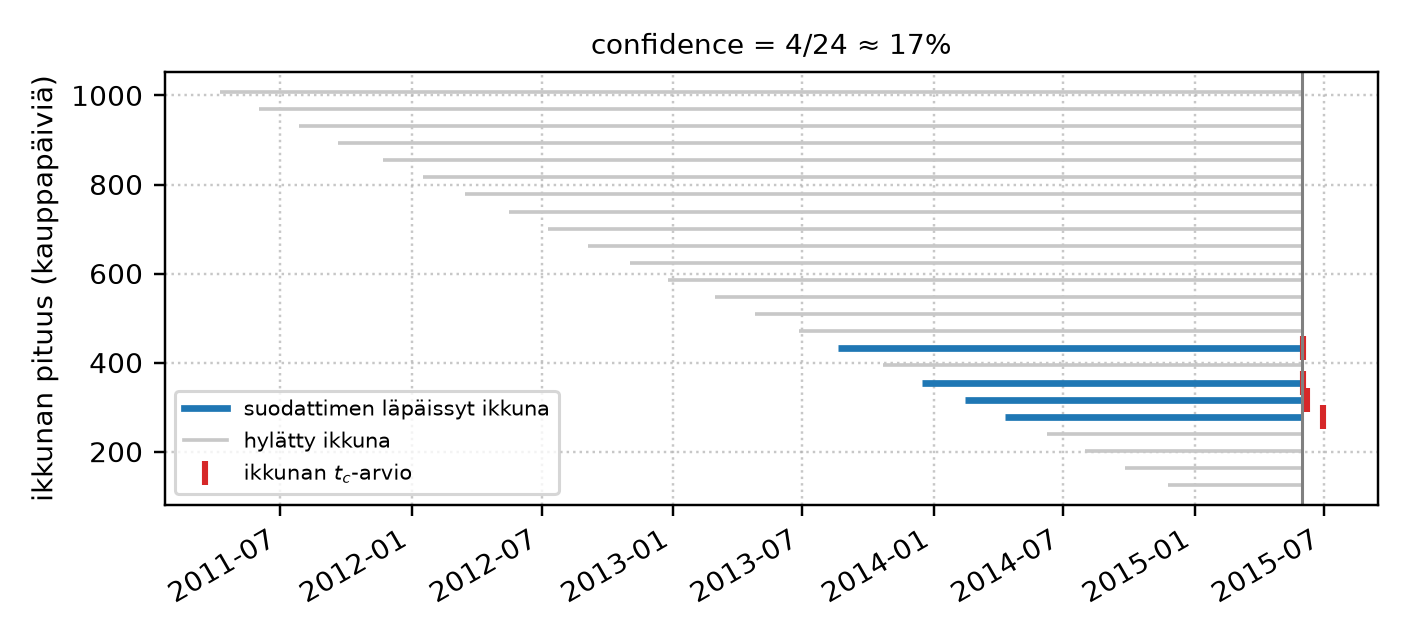
\includegraphics[width=0.72\textwidth]{kuva3_ikkunat.png}
  \caption{Samat tiedot ikkunoittain. Jokainen vaakaviiva on yksi sovitusikkuna, joka päättyy
    1.6.2015. Sinisten ikkunoiden sovitukset läpäisivät suodattimen, ja punaiset merkit ovat
    niiden $\tc$-arviot. Luottamusindikaattori oli $4/24 \approx 17\,\%$. Jokainen ikkuna vastaa
    noin neljää prosenttiyksikköä, joten kuplan raja 10\,\% vaatii vähintään kolme hyväksyttyä
    ikkunaa.}
  \label{fig:ikkunat}
\end{figure}

% ---------------------------------------------------------------------------
\section{Kuplan havaitsemisen ehdot}\label{sec:ehdot}

\subsection{Sovituksen suodatin}\label{sec:suodatin}

Optimointi löytää aina jonkin parhaan sovituksen myös satunnaisesta sarjasta. Siksi jokainen
sovitus tarkistetaan ehdoilla, jotka sulkevat pois fysikaalisesti mielettömät ja
tilastollisesti heikot sovitukset. Värähtelyjen voimakkuutta suhteessa trendiin mittaa
vaimennus (\emph{damping}), ja värähtelyjen määrää ikkunassa puolijaksojen lukumäärä:
\begin{equation}\label{eq:damping}
  D = \frac{m\,|B|}{\omega\,|C|},\quad |C|=\sqrt{C_1^2+C_2^2},\qquad\qquad
  O = \frac{\omega}{\pi}\ln\frac{\tc-t_1}{\tc-t_2}.
\end{equation}
Sovituksen tarkkuutta mitataan log-hinnan jäännösten neliökeskiarvolla
\begin{equation}\label{eq:rmse}
  \mathrm{RMSE} = \sqrt{\frac{1}{N}\sum_{i=1}^{N}\left(y_i-\hat y_i\right)^2}.
\end{equation}
Taulukossa~\ref{tab:suodatin} ovat sovelluksen käyttämät rajat. Ehto $D \ge 1$ takaa likimain,
että yhtälön~\eqref{eq:hazard} riskifunktio pysyy ei-negatiivisena. \citet{zhang2016} käyttävät
tätä rajaa, mutta tämän sovelluksen kalibroinnissa se hylkäsi seitsemän kahdeksasta tunnetusta
kuplasta. Siksi käytössä on Wheatleyn ym.\ \citeyearpar{wheatley2019}
Bitcoin-tutkimuksen raja $D \ge 0.5$ ja sen väljempi $\omega$-alue. Ehto $O \ge 2.5$ estää mallia
selittämästä yksittäistä heilahdusta \enquote{värähtelyksi}.

\begin{table}[htbp]
  \centering\small
  \begin{tabularx}{\textwidth}{@{}l l X@{}}
    \toprule
    Ehto & Raja & Peruste ja lähde \\
    \midrule
    eksponentti $m$ & $0.1 < m < 0.9$ & kasvu kiihtyy, mutta hinta pysyy äärellisenä \citep{zhang2016} \\
    log-taajuus $\omega$ & $4 < \omega < 25$ & realistinen värähtely \citep{wheatley2019} \\
    vaimennus $D$ & $D \ge 0.5$ & värähtelyt eivät hallitse trendiä \citep{wheatley2019} \\
    puolijaksot $O$ & $O \ge 2.5$ & aitoa värähtelyä, ei kohinaa \citep{zhang2016} \\
    kriittinen hetki & $t_2 < \tc \le t_2 + 0.13\,\Delta t$ & ennuste on lähellä ja tulevaisuudessa \citep{zhang2016} \\
    sovitusvirhe & $\mathrm{RMSE} \le 0.15$ & kalibroitu testikuplilla; kryptovaluutat ovat volatiileja \\
    suunta & $B<0$ / $B>0$ & kupla / antikupla \\
    \bottomrule
  \end{tabularx}
  \caption{Yksittäisen sovituksen hyväksymisehdot.}
  \label{tab:suodatin}
\end{table}

\subsection{Hinnannousun ehto}

LPPLS-muoto voi löytyä myös hitaasta ja vaatimattomasta noususta. Kuplalta edellytetään siksi
lisäksi suurta toteutunutta nousua. \citet{greenwood2019} tutkivat toimialaportfolioita vuosilta
1926--2014. Kun nousu kahden vuoden aikana oli 100\,\%, 40\,\%:n romahduksen todennäköisyys
seuraavien kahden vuoden aikana oli noin 53\,\%. 50\,\%:n nousulla todennäköisyys oli noin
20\,\%. Sovellus laskee nousun kahden vuoden pohjasta:
\begin{equation}\label{eq:runup}
  R(t_2) = \frac{p(t_2)}{\displaystyle\min_{t_2-730\pv\,\le\, t\,\le\, t_2} p(t)} - 1 .
\end{equation}
Kuplalta vaaditaan $R \ge 1$ eli hinnan kaksinkertaistuminen. Antikuplalta vaaditaan vastaavasti
vähintään 50\,\%:n lasku kahden vuoden huipusta. Log-asteikolla molemmat ovat yhtä suuria
muutoksia ($\ln 2$).

\subsection{Luokittelu ja seuranta}

Lopullinen luokitus yhdistää luottamusindikaattorin ja hinnannousun
(taulukko~\ref{tab:luokat}). Kuplaksi luokiteltu tilanne tallennetaan tietokantaan.
Tallennettava ennuste jäädytetään: parametreja ei myöhemmin päivitetä, vaan ennustetta verrataan
uuteen dataan. Seurannassa etsitään huippu $t^*$ havaintopäivän ja ennustevälin lopun välistä.
Kupla on \emph{toteutunut}, jos huippua seuraa 90 päivän sisällä vähintään 15\,\%:n pudotus, eli
$1 - \min_s p(s)/p(t^*) \ge 0.15$. Tila on \emph{ei toteutunut}, jos ennusteväli (vähintään
$\pm 30$ päivää) ohitetaan ilman pudotusta, ja muuten \emph{odottaa}.

\begin{table}[htbp]
  \centering\small
  \begin{tabularx}{\textwidth}{@{}l X l@{}}
    \toprule
    Tila & Ehdot & Toiminto \\
    \midrule
    kupla & $\mathrm{CI} \ge 10\,\%$, mediaani-$\tc \le 6$~kk ja $R \ge 100\,\%$ & tallennus ja seuranta \\
    lähellä & $\mathrm{CI} \ge 5\,\%$ ja $R \ge 50\,\%$ & näytetään taulukossa \\
    ei & muut & -- \\
    \bottomrule
  \end{tabularx}
  \caption{Skannauksen luokittelu.}
  \label{tab:luokat}
\end{table}

% ---------------------------------------------------------------------------
\section{Kalibrointi ja rajoitukset}\label{sec:kalibrointi}

Raja-arvot valittiin kokeilemalla eri yhdistelmiä kahdeksalla historiallisella kuplalla ja
yhdellätoista vertailutapauksella (taulukko~\ref{tab:testit}). Kuusi kahdeksasta kuplasta
tunnistui, eikä yksikään vertailutapaus luokittunut kuplaksi. Vertailutapauksia olivat S\&P 500
vuosina 2007 ja 2019, DAX 2014 sekä yhdeksän indeksiä lokakuussa 2026, joista S\&P 500 ja NYSE
FANG+ luokittuivat tilaan \enquote{lähellä}. Kriittisen hetken arvio osui 0--4 viikon päähän
todellisesta huipusta. Nikkei 1989 jäi tunnistamatta, koska sen nousu kahdessa vuodessa oli vain
69\,\%. Bitcoin maaliskuussa 2021 jäi tunnistamatta, koska vain harva ikkuna läpäisi
suodattimen.

\begin{table}[htbp]
  \centering\small
  \begin{tabular}{@{}l r r l l l@{}}
    \toprule
    Tapaus (tarkastelupäivä) & CI & Nousu 2 v & Tulos & Ennuste $\tc$ & Todellinen huippu \\
    \midrule
    Bitcoin 1.12.2017      & 17\,\% & $+2956\,\%$ & kupla & 4.12.2017  & 16.12.2017 \\
    Shanghai 1.10.2007     & 13\,\% & $+414\,\%$  & kupla & 31.10.2007 & 16.10.2007 \\
    Shanghai 10.10.2007    & 17\,\% & $+435\,\%$  & kupla & 26.10.2007 & 16.10.2007 \\
    Shanghai 1.6.2015      & 17\,\% & $+148\,\%$  & kupla & 5.6.2015   & 12.6.2015 \\
    Nasdaq 15.2.2000       & 25\,\% & $+212\,\%$  & kupla & 16.2.2000  & 10.3.2000 \\
    Nasdaq 1.3.2000        & 38\,\% & $+237\,\%$  & kupla & 4.3.2000   & 10.3.2000 \\
    Nikkei 225 15.11.1989  & 0\,\%  & $+69\,\%$   & ei    & --         & 29.12.1989 \\
    Bitcoin 15.3.2021      & 4\,\%  & $+1311\,\%$ & ei    & --         & 13.4.2021 \\
    \bottomrule
  \end{tabular}
  \caption{Historialliset testikuplat nykyisillä ehdoilla.}
  \label{tab:testit}
\end{table}

Tuloksia on tulkittava varoen. Rajat valittiin samoilla tapauksilla, joilla niitä testattiin,
joten osuvuus uusilla aineistoilla on todennäköisesti heikompi. Parametri $\tc$ on tunnetusti
huonosti määräytyvä: kuplan alku on helpompi tunnistaa kuin sen loppu, ja eri ikkunat antavat
hajanaisia arvioita \citep{zhang2016}. Malli kuvaa sisäsyntyisiä kuplia, joten se ei ennakoi
ulkoisia shokkeja kuten pandemiaa tai sotaa. Kupla voi myös päättyä hitaaseen laskuun. Lisäksi
Yahoo Financen data voi sisältää puutteita. Sovellus on tarkoitettu tutkimus- ja
opiskelukäyttöön, eikä sen tulos ole sijoitussuositus.

% ---------------------------------------------------------------------------
\begin{thebibliography}{9}
\small
\setlength{\itemsep}{2pt}

\bibitem[Filimonov ja Sornette(2013)]{filimonov2013}
Filimonov, V. \& Sornette, D. (2013). A stable and robust calibration scheme of the log-periodic
power law model. \emph{Physica A}, 392(17), 3698--3707.

\bibitem[Greenwood ym.(2019)Greenwood, Shleifer ja You]{greenwood2019}
Greenwood, R., Shleifer, A. \& You, Y. (2019). Bubbles for Fama. \emph{Journal of Financial
Economics}, 131(1), 20--43. \url{https://www.nber.org/papers/w23191}

\bibitem[Johansen ym.(2000)Johansen, Ledoit ja Sornette]{johansen2000}
Johansen, A., Ledoit, O. \& Sornette, D. (2000). Crashes as critical points.
\emph{International Journal of Theoretical and Applied Finance}, 3(2), 219--255.

\bibitem[Johansen ja Sornette(2010)]{johansen2010}
Johansen, A. \& Sornette, D. (2010). Shocks, crashes and bubbles in financial markets.
\emph{Brussels Economic Review}, 53(2), 201--253. \url{https://arxiv.org/abs/cond-mat/0210509}

\bibitem[Nelder ja Mead(1965)]{nelder1965}
Nelder, J.\,A. \& Mead, R. (1965). A simplex method for function minimization.
\emph{The Computer Journal}, 7(4), 308--313.

\bibitem[Sornette(2003)]{sornette2003}
Sornette, D. (2003). \emph{Why Stock Markets Crash: Critical Events in Complex Financial
Systems}. Princeton University Press.

\bibitem[Wheatley ym.(2019)Wheatley, Sornette, Huber, Reppen ja Gantner]{wheatley2019}
Wheatley, S., Sornette, D., Huber, T., Reppen, M. \& Gantner, R.\,N. (2019). Are Bitcoin bubbles
predictable? Combining a generalized Metcalfe's law and the log-periodic power law singularity
model. \emph{Royal Society Open Science}, 6(6), 180538. \url{https://arxiv.org/abs/1803.05663}

\bibitem[Zhang ym.(2016)Zhang, Zhang ja Sornette]{zhang2016}
Zhang, Q., Zhang, Q. \& Sornette, D. (2016). Early warning signals of financial crises with
multi-scale quantile regressions of log-periodic power law singularities. \emph{PLoS ONE},
11(11), e0165819. \url{https://doi.org/10.1371/journal.pone.0165819}

\end{thebibliography}

\end{document}
